\documentclass[12pt]{cpa2015}
% To produce camera-ready copy with no running headers, etc., add the
% "crc" option above (i.e. \documentclass[12pt,crc]{...}).

\usepackage{times}
%\usepackage[T1]{fontenc}
\usepackage{url}
\usepackage{bold-extra}
\usepackage{algpseudocode}
\usepackage{tikz}
\usetikzlibrary{fit}
\usepackage{tkz-kiviat}
\usepackage{todonotes}

\usepackage{color}
\usepackage{float}
\usepackage{sidecap}

\usepackage{cpalistings}

\normalfont

\begin{document}
\begin{frontmatter}

\setcounter{page}{1}


\title{A Design for Interchangeable\\Simulation and Implementation}
\runningtitle{A Design for Interchangeable Simulation and Implementation}

\author{\fnms{Klaus} \fnms{Birkelund} \snm{JENSEN}}~~and~~\author{\fnms{Brian} \snm{VINTER}}
%\runningauthor{Jensen et al.}
\address{Niels Bohr Institute, University of Copenhagen, Denmark\\[4pt]%
	{\small \{{\tt birkelund}~,~{\tt vinter\}{\tt @nbi.ku.dk}}}
}

\begin{abstract}
Research on concurrent systems requires modeling, simulation and
evaluation in many settings. We describe a design for Interchangeable
Simulation and Implementation (ISI, pronounced \emph{easy}), an approach that enables the simultaneous
modeling, simulation and evaluation of highly concurrent process based systems.

We describe how ISI can been used to design and evaluate techniques used in
storage systems. Our key insight is that, while the simulation of systems could
be implemented as regular discrete event simulation, the benefits of designing
it as the highly concurrent process based system that it is --- with the full data
and control flow in mind --- enables seamless interchangeability between
discrete and real time simulation.
\end{abstract}

\begin{keyword}
design patterns\sep
concurrent process architectures\sep
systems simulation and modeling
\end{keyword}
\end{frontmatter}

\section*{Introduction}
Research on large-scale storage systems in relation to energy consumption is
an increasingly active area with many recent developments\cite{survey-power}. This is
motivated by the fact that storage needs are increasing rapidly and
exponentially in the data center and thus the energy bill associated
with storage becomes a relatively large part of running an I/O intensive
business.

Much of this research has focused on methods and techniques for optimizing
existing storage and file systems; especially in the area of power-aware
RAID\cite{paraid} or similar energy-efficient and durable storage. To this end,
we are developing a system that allows us to simulate, prototype and validate
the implementation of a storage system.  That system is not the topic of this
paper, but serves as an important case study and context in which we will
present the concurrent architecture (or \emph{design pattern}), called
Interchangeable Simulation and Implementation (ISI), that we have identified
while developing the simulator. Our system should be a power-aware simulator at
large-scale and provide us with designs for storage hierarchies, but we wanted
to decrease the time between simulation (\emph{design}) and prototyping
(\emph{implementation}) of the designs. Similarly we wanted to allow a form of
validation through measurements of the model.

First, this paper presents some background and our motivation is described in
context of related work on systems and storage simulation. Next, the
architecture is described followed by a description of how ISI can be used to
effectively develop highly concurrent systems that can be simulated, prototyped
\emph{and} validated using a single toolbox.

\section{Background}
Most work in the field of storage system simulation is based on Discrete
Event Simulation (DES) such as Eeffsim\cite{eeffsim}, a simulator for energy
efficiency of large-scale storage systems. DES have broad applications and are
commonly used when studying queuing in traffic,
maritime, military and network simulations\cite{omnetpp}. They are relatively
easy to implement as they basically consist of the main loop represented in
algorithm~\ref{des-main-loop}. Note that $Q$ is kept sorted in order
of decreasing virtual time stamp.

\begin{algorithm}[H]
	\caption{Discrete Event Simulation (main loop)}
	\label{des-main-loop}
	\begin{algorithmic}[1] % The number tells where the line numbering should start
		\Procedure{DES-LOOP}{$Q$}
		\While{$Q\neq\emptyset$}
		\State $e \gets \Call{Dequeue}{Q}$
		\State $T \gets \Call{Clock}{e}$ ~~~~~~~~$\triangleright$ Update world clock
		\State $\Call{Process}{e}$ ~~~~~~~~~~~~~~$\triangleright$ Process event and enqueue new
		\EndWhile
		\EndProcedure
	\end{algorithmic}
\end{algorithm}

A DES is essentially a priority queue from which the oldest events are popped
as the simulation progresses. Note that each processing step may add one or
more events to the queue. This works well as
long as the simulator is single-threaded, but it is not easily parallelized.
This stems from the discrete nature of the algorithm. The single crucial
invariant that must hold is that we always pop the event with the lowest time
stamp. In Parallel Discrete Event Simulation (PDES), DES is generalized
by providing each logical process (e.g. an airport, an aircraft or a
passenger) with its own priority queue of events to handle and the different
processes communicate by sending events to each other. This decomposition leads
to the problem of causality violations. We define causality to be the fact that
the past cannot be changed, such that a violation occurs if at time $t_i$ an
event influences something at time $t_j$, where $t_j < t_i$. The two main
approaches to PDES handle this issue differently. While the \emph{conservative}
approach introduces an ancillary communication round-trip (called
\emph{null}-messages) to ensure no
causality violation happens if the current event candidate is
handled\cite{conservative-pdes-1, conservative-pdes-2}, the \emph{optimistic}
approach requires the user of the simulator to provide \emph{reverse} handlers
that are called if a violation is discovered\cite{timewarp}. In optimistic
simulators, this can cause a cascade of reverse calls, and some applications
can simply not be implemented using an optimistic PDES\cite{fujimoto-pdes}.

We emphasize discrete event simulation, because it is in this area where ISI
exhibits some advantages over traditional methods. While there are arguably
many methodologies one can follow when developing applications and large-scale
systems, ISI is designed to be used in a domain where the system under
consideration is not completely understood. In our context, part of this is the
hierarchical structure of a scalable storage system. While the functional
behaviour of the various system parts (i.e tape drives, hard drives and
prefetchers) are well-known, the delicate interactions and their consequences
are not. To that end, we opted for a methodology centered around simulation,
prototyping and analysis:

\begin{enumerate}
	\item \emph{Simulate} a model and identify a design.
	\item \emph{Implement} a prototype from the design.
	\item \emph{Measure} the prototype and \emph{validate} it and the model
		against predictions.
	\item \emph{Repeat}. Feed the results of the validation back into the
		simulator and/or model and repeat from step 1.
\end{enumerate}

Alas, this is a cumbersome iterative process. While the iterative process is
completely sound, we will argue that the tedious work on prototype
reimplementation and/or refactoring can be eliminated. Similarly, we will argue
that simulation and measurement can be combined and finally arguing that one
system can encompass all of the above by adhering to the ISI architecture.

\subsection{Related Work}
ROSS\cite{ross} is a massively parallel discrete-event simulation tool for the
modeling of very large scale systems. It is an optimistic simulator that uses
the Time Warp\cite{timewarp} protocol for synchronizing the global clock. ROSS
has recently\cite{ross-warpspeed} been shown to run on an extremely large number of
processors\footnote{1,966,080 cores.} using the Message
Passing Interface\cite{mpi}. SimPy\cite{simpy} is a process-based discrete
event simulation framework written
in Python. It allows simulation in discrete and real-time and uses Python
\emph{generators} to implement ``processes''.

ISI shares ideas with the notion of \emph{micro
services}\cite{microservices}, recently popularized.
The micro service architecture is motivated by some of the same issues, though
primarily rooted in the area of distributed computing and the effectiveness of
being loosely coupled in relatively chaotic and inhospitable settings.

ISI can also be compared to that of flow-based programming\cite{flowprog} where
applications are defined as a network of \emph{black box} processes, allowing
these processes to be reconnected in various ways, sometimes dynamically.


\subsection{Differences and Comparisons}
\label{sec:diff-comp}
To illustrate the main differences between a PDES and our approach, consider a
network of airports in which we want to model aircraft arrivals and departures
with a limited number of runways available at each airport. In a PDES approach,
the interactions are modeled as events, i.e. \verb|arrival|, \verb|departure|
and \verb|landing|. One airport may receive and act on a \verb|landing| event and
immediately schedule a \verb|departure| event with itself, which would again
schedule an \verb|arrival| event at another airport. Here, the airport
represents a process, but the aircraft, passengers etc. are just state. In a
concurrent setup, the risk of violating causality is high in optimistic
simulators. To see this, consider an airport $A$, and let $t(x)$ denote the
associated local clock (or in the case of events, the time stamp) of $x$. Under
normal circumstances, $A$ will process incoming events $e_i$ such that $t(e_1)
< t(e_2) < \dots < t(e_n)$. After processing an event, the local clock $t(A)$
is updated, such that $t(A) = t(e_i)$. Now, causality violations happen in the
case where an event $e_k$ originates from airport $B$ and is received such that
$t(e_k) < t(A)$. In optimistic PDES, $A$ must now call reverse handlers for all
locally processed events $e_i$ with $t(e_i) > t(e_k)$, then call handler for
$e_k$ and then reapply handlers for all events that were reversed. This can
lead to the cascade of event reversals previously mentioned.

It follows from the above, that in PDES, an event $e_i$ is already scheduled to
happen at some time $t(e_i$) when it is created. This is a central concept of
(P)DES. In ISI, we take a different approach. We no longer pass events around,
but exchange messages (or aircraft) as the system would do in the real world.
With ISI, processes are used to model anything that could be regarded as a
process. In our airport example, the \emph{sky} is a process that should handle
aircraft traffic and determine flight durations when \emph{receiving} an
aircraft and \emph{sending} it to its destination, calculating the flight time
by exchanging messages with the two airports involved. Note though, that the
sky now becomes a bottleneck if left as a single process. There are various
ways of distributing this process while maintaining causality such as barrier
synchronization\emph{phases}\cite{birds}, but a discussion of that
is out of scope for this paper.
%This fact leads us to an important distinction
%between PDES and ISI.

Protection against causality violations is \emph{not} implicitly provided by
ISI. This is justified by the fact
that requirements on ordering are largely domain specific. For some systems, a
logical vector clock\cite{lamport-time} imposing a partial ordering might be
good enough. For others, a globally synchronized clock\cite{timewarp} could be
essential. Instead of imposing a specific time handling, we rely on the
developer to handle this. At first glance, this might seem like a harsh
requirement, but the case study in section~\ref{sec:case-study} will show how this relaxation can
be used to simplify time handling in systems that do not need exact time
keeping. Or, as in the case study, only requires relative time handling.

The process-oriented programming model of ISI, where individual logical
processes interact by messaging each other through communication
\emph{channels}, have been formalized by process algebras such as CSP\cite{csp}
and the $\pi$-calculus\cite{pi-calculus}. The real world is highly concurrent
and process calculi ensures that communication semantics and process
composition are well-defined. Furthermore, the programming model ensures that a
design can be made to run in a distributed setting without much refactoring due
to the implicit share-nothing architecture that it represents. In the context
of storage system simulation, such systems map to independently interacting
processes, usually organised in a tree. Process-based modeling has already
been used in many other systems, e.g. CoSMoS\cite{cosmos} and agent-based PDES
approaches\cite{agent-based-pdes}.

The Kiviat diagram in figure~\ref{kiviat} is our comparison of DES, PDES and ISI. We
examine the areas of Flexibility, Performance, Clarity and Composability. The
diagram primarily serves to show our goals for ISI and where we believe the
design pattern has advantages over other methods. We regard ISI as much more
flexible and clear than DES and PDES. In particular, components are easily
composed when using the ISI architecture, yielding a high score on Flexibility
and Composability. For Clarity, the processes used in ISI are straight-forward
implementations of real-world logic. This is compared to both DES and PDES, but
especially PDES lacks clarity, due to reverse handlers for instance. We note
though, that PDES has a very high score on raw performance. Raw performance is
not the immediate goal for ISI, but as we shall see in
section~\ref{sec:results}, performance is reasonable, though no
quantitative comparison has been done against PDES.


\begin{figure}[htb]
\begin{tikzpicture}
	\tkzKiviatDiagram[
		radial=4,
		lattice=5,
		radial  style/.style ={.}
			%lattice style/.style ={blue!30}
	]{\emph{Clarity},\emph{Flexibility},
	\emph{Performance},\emph{Composability}}
	\tkzKiviatLine[ % ISI
		thick,
		color=black,
		fill=black!20
	](4,4,2,4)
	\tkzKiviatLine[ % DES
		densely dotted,
		color=black,
		fill=black!40
	](3,2,1,1)
	\tkzKiviatLine[ % PDES
		loosely dotted,
		color=black,
		fill=black!60
	](1,1,5,1)

\end{tikzpicture}
\caption{A comparison of ISI (lighter, solid), DES (densely
	dotted) and PDES (darker, loosely dotted).}
\label{kiviat}
\end{figure}



\section{High Productivity with ISI}
The goal of ISI is to allow the simultaneous \emph{simulation},
\emph{prototyping} and \emph{validation} of a system during development.
Figure~\ref{easy} illustrates the ISI method on a high level. Like the
four-step development method described in the previous section, ISI includes
simulation, prototyping and measurement, but design, implementation and
validation are implicit by-products. In section~\ref{sec:case-study}, we shall see an example on
how this can be achieved. An essential requirement of ISI is that the real world
is modeled \emph{as is}. This, of course, is usually not possible, but domain
specific abstractions apply as in all models. This requirement stems from the
fact that in order for the components of the simulation to be usable as
prototypes, they should implement \emph{real-world} logic as much as possible.

\begin{figure}[htb]
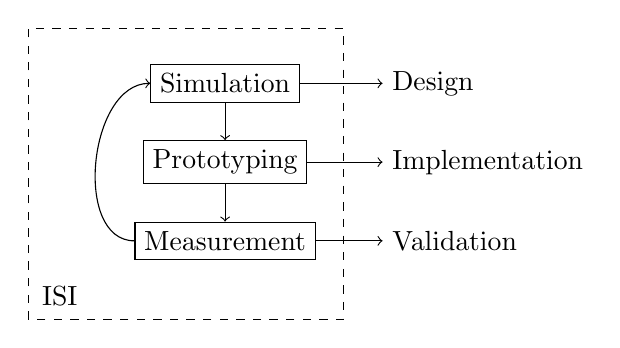
\begin{tikzpicture}
	\node[draw] (Simulation) at (0,2) {Simulation};
	\node[draw] (Prototyping) at (0,1) {Prototyping};
	\node[draw] (Measurement) at (0,0) {Measurement};

	\node (ISI) at (-2.1,-.7) {ISI};
	\draw[dashed] (-2.5,-1) -- (-2.5,2.7) -- (1.5,2.7) -- (1.5,-1) -- (-2.5,-1);

	\node[anchor=west] (Design) at (2,2) {Design};
	\node[anchor=west] (Implementation) at (2,1) {Implementation};
	\node[anchor=west] (Validation) at (2,0) {Validation};

	\draw[->,draw] (Measurement) to[in=180,out=180] (Simulation);
	\draw[->,draw] (Simulation) to (Design);
	\draw[->,draw] (Prototyping) to (Implementation);
	\draw[->,draw] (Measurement) to (Validation);

	\draw[->,draw] (Simulation) to (Prototyping);
	\draw[->,draw] (Prototyping) to (Measurement);
\end{tikzpicture}
\caption{A high-level description of the ISI architecture}
\label{easy}
\end{figure}

\subsection{Process-based Modeling}
For ISI to be applicable the model must be decomposed into distinct and
independently communicating parties or \emph{processes}. As the world is highly
concurrent, decomposition is rarely an issue, but the inverse is. Limiting
concurrency is an issue that PDES approaches must deal with, customarily done
by mapping multiple \emph{physical} processes to one \emph{logical} process.
This has the disadvantage of coupling the previously distinct processes. This can
often be optimized, but still represents an engineering challenge.

In the context of a storage system, a natural decomposition into distinct
processes is ``simply'' to identify the concurrent interactions that take
place, i.e. the issuing of I/O requests from clients, handling by a cache, the
latency introduced by switches etc.

For ISI to be effective, an environment that allows millions of concurrent
processes is required. This can be achieved through direct language support
(such as present in Erlang\cite{erlang}, Go\cite{Go} or
occam-$\pi$\cite{occam-pi}) or through libraries such as ZeroMQ\cite{zeromq} for
languages lacking direct support. Here, we employ Go, which is Google's
emerging concurrent programming language. Go is in part influenced from C,
occam, Limbo\cite{limbo} and Newsqueak\cite{newsqueak} and includes
language-level concurrency primitives such as light-weight processes called
\emph{goroutines}, first-class communication channels and the
\verb|select|-statement which allows non-deterministic choice
(pseudo-random) from a set of possible send or receive operations. Go is
designed to be highly productive and easy to learn. It does so, by promoting
convention over convenience and using a relatively small number of syntactic
elements compared to e.g. C++. Go is generally not considered to be an
object-oriented language, and uses another approach compared to other
languages. Methods are allowed on \emph{any} type and does not use the notion
of a \emph{class}. To implement dynamic dispatch, Go provides \emph{interface}
types that are compatible with any type implementing the methods described in
the interface\cite{goref}.

While the concurrency features of Go were influenced from CSP and the $\pi$-calculus,
it cannot be uniquely categorized. The concurrency features are often discussed
in the context of CSP, but Go's channels are more akin to the $\pi$-calculus
because channels may be communicated over channels. On the other hand, Go does not
allow guards in \verb|select|-statements.

To an observer the different processes are completely sequential and blocking
in nature. The process receives a message, handles it and (optionally)
replies with an answer. We find that this programming model is simpler to
understand than what is known as the \emph{callback hell}\cite{callback-hell} arising from
asynchronous single-threaded event handling, known from building concurrent
services in languages that don't provide light-weight process support (e.g.
JavaScript).

\subsection{Tracking Time}
\label{sec:tracking-time}
As described in section~\ref{sec:diff-comp}, ISI does not impose any specific
method for tracking time, but for ISI to be applicable to a broad range of
systems, we need to discuss how to handle causality. We are not interested in
ever handling reverse events as is needed in the previously mentioned Timewarp
PDES algorithm.  Doing so would eliminate the point of ISI; that simulation and
implementation is interchangeable. A prototype should not have to handle a
causality violation. It won't happen in real life.

Instead, some concepts from conservative PDES are elegant solutions for
communicating processes. Given a process $p$, that handles
requests for connected peers $a_i$, one approach is to ensure that all $a_i$
always has at least one message queued at $p$. These messages can be actual
requests, or if the process is simulating a period of inactivity, a
message indicating the how long. This ensures that $p$
can handle requests for all remaining processes, without violating causality,
but does require a process' peers to be static. The technique is not as
straight-forward as it sounds and does require special \emph{null}-messages
(with no other purpose than updating a clock) to avoid deadlocks. The
conservative PDES approach in general, as well as why \emph{null}-messages are
required to avoid deadlocks, are beyond the scope of this paper, but see Misra's
1986 paper\cite{dist-des} for a thorough description and proof of correctness.

While the conservative approach is universal and could be built into an ISI
library, we will argue in section~\ref{sec:case-study}, that not all
simulations or systems require these extra messages, justifying our choice that
ISI should not handle causality implicitly.

\subsection{Simulation as Measurement}
A distinctive feature of ISI is that real-time measurement is done at the same
points as where simulation happens. The only change needed to transition from
simulation to measurement is to swap the randomized timings common in event
simulations with an actual timing around an actual operation. This
substantially decreases the time from simulating a system to testing a
prototype in the lab because the prototype is implicitly designed and
implemented through the development of the simulator.

The implicit support for measurement in the prototype also makes testing and
verifying the system model uncomplicated and ensures that the final system is
capable of doing statistics at reference points which, through simulation, was
found to be important for reasoning about the system.

Similarly, as described in section~\ref{sec:tracking-time}, periods of
inactivity are handled in simulation by sending messages about inactivity to
peers. An action that is simply disabled when moving to measurement, because
this is now handled by actual waiting for resources or replies.

\subsection{Validation}
In our storage simulator, a workload generator produces a stream of synthetic
I/O requests. As the simulator evolves, so does a system capable of handling
these I/O requests in a real setting. To validate and reason about the
precision of the simulation, simulated actions of components can be gradually
swapped for real actions. The result of processing request in real-time
provides valuable feedback to our software such that simulated durations can
be tuned.  This is the iterative process that was described in the introduction.

Thus, validation can be regarded as part of the development work flow, but it
does not require a separate validation engine; the built-in measurements are
sufficient.

\section{A Case Study}
\label{sec:case-study}

%\begin{figure}[htb]
%\begin{tikzpicture}
%	\node[draw] (drive0) at (0,0) {$drive_0$};
%	\node[draw] (drive1) at (2,0) {$drive_1$};
%	\node (driveDots) at (4,0) {$\dots$};
%	\node[draw] (driveN) at (6,0) {$drive_n$};
%
%	\draw (drive0) -- (0,-1);
%	\draw (drive1) -- (2,-1);
%	\draw[dashed] (driveDots) -- (4,-1);
%	\draw (driveN) -- (6,-1);
%	\draw (0,-1) -- (6,-1);
%
%	\draw (3,-1) -- (3,-2);
%
%	\node[draw] (changer0) at (0,-3) {$changer_0$};
%	\node[draw] (changer1) at (2.5,-3) {$changer_1$};
%	\node (changerDots) at (4.2,-3) {$\dots$};
%	\node[draw] (changerN) at (6,-3) {$changer_n$};
%
%	\draw (changer0) -- (0,-2);
%	\draw (changer1) -- (2.5,-2);
%	\draw[dashed] (changerDots) -- (4.2,-2);
%	\draw (changerN) -- (6,-2);
%
%	\draw (0,-2) -- (6,-2);
%
%	\node[draw] (client0) at (10,0) {$client_0$};
%	\node[draw] (client1) at (10,-1) {$client_1$};
%	\node (clientDots) at (10,-2) {$\dots$};
%	\node[draw] (clientN) at (10,-3) {$client_n$};
%
%	\draw (client0) -- (8,0);
%	\draw (client1) -- (8,-1);
%	\draw[dashed] (clientDots) -- (8,-2);
%	\draw (clientN) -- (8,-3);
%
%	\draw (8,0) -- (8,-3);
%\end{tikzpicture}
%\caption{Overview of the tape library architecture.}
%\label{easy}
%\end{figure}

To illustrate an ISI architecture, this section will describe a tape library
simulation. This example does not use any library support (except the Go
standard library) and serves to show how a large-scale tape system can be
simulated in a highly concurrent environment in a relatively simple manner.

A large-scale tape system (or \emph{library}) consists of a number of tape
drives and one or more robots (or \emph{changers}). Our example simulates
low-level client access to the library by instructing the changer to mount a
tape in a drive and, when ready, issue I/O requests directly to the drive.
While this is obviously a simple example, it does, however, reflect how clients
interact with a tape library in a \emph{real-world} manner.

The example is also meant to highlight the instinctive implementation. The
system includes three types of processes: changers, drives and clients. They
are implemented to behave as the real-world process that they model. This means
that they wait when they would in the real world and the code generally flows
as one would implement an actual library controller.

An important and distinctive feature of ISI is that mutual exclusion is
implicitly ensured. For instance, a drive must only be allocated to and used by
\emph{one} client at a time. This sequentiality is trivially provided due to
the sequential nature of the processes. This, of course, is not a feature
unique to ISI, but for any communicating process architecture. For any
process-based architectures this is a benefit resulting from explicitly
disallowing any sharing of data; a so-called
\emph{share-nothing} architecture.



Listing~\ref{basic-types} shows the basic types that are used in the
simulation\footnote{Full source code available at
\url{http://github.com/kbj/papers/cpa15/src}}. All requests carry a command
(\verb|mount|,
\verb|unmount|, \verb|read|, etc.), as well as a \verb|response|
channel to reply on. Similarly, the \verb|response| contains the duration
of the operation, as well as an optional \verb|request| channel. The
purpose of this channel is to	enable one-to-one communication between two
processes explicitly.

\begin{lstlisting}[caption={Basic types for tape simulation}, label=basic-types]
type request struct {
    cmd   command
    ch    chan response
    clock time.Time
}

type response struct {
    t     time.Duration
    ch    chan request
    clock time.Time
}

type library struct {
    changers chan request
    drives   chan request
}
\end{lstlisting}

Here, the library basically consists of two any-to-any channels. Changers and
drives receive messages on those two channels respectively, but never write to
them. Messages sent on Go channels do not carry a destination, so replies would
not end up with the original sender if written to the channel.


The code in these listings uses \emph{rendezvous-style} communication channels
as in CSP. Go has support for asynchronous messaging (through buffered
channels) and the performance results in section~\ref{sec:results} includes
results where this has been used. Inappropriate buffering could impact the
causality constraints or correctness, because the use of buffered channels
might cause a process to think that a message has been handled even though it
still lingers in the channel buffer. To avoid this, we employ a request/reply
idiom common in the Go community where we exploit the ability to communicate
channels along the channels themselves as in the $\pi$-calculus. Being able to
pass a channel to another process is useful as it allows the process to create a
dedicated \emph{reply} channel for a single request, ensuring that no other
communication will happen until the unique response is received. The code in
listing~\ref{reqresp} shows how this can be done, and
figure~\ref{reqresp-illustration} illustrates how this is employed in our
simulation to chain multiple processes. The request and response messages
exchanged are represented by \lstinline{req} and \lstinline{resp} respectively.
In general the messages carry a payload, which for requests are the channel a
reply should be directed to. For responses the payload is a channel that can be
used for further communication, but may (as in step 6 of
figure~\ref{reqresp-illustration}) exclude this to indicate that no further
communication is expected.
%Similar techniques are outlined in\cite{dyn-proc-net-go}.


\begin{lstlisting}[caption={Request/response using Go channels},label={reqresp}]
func request(ch chan response) {
    go func() { ch <- response{} }()
}

func client() {
    ch := make(chan response)
    request(ch);    // start work in goroutine
    <-ch            // wait for completion
}
\end{lstlisting}

\begin{figure}[htb]
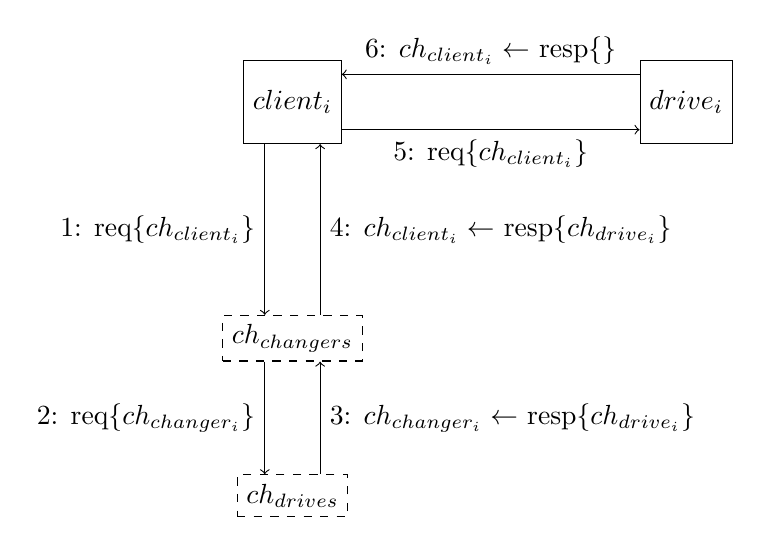
\begin{tikzpicture}
	\node[draw,minimum size=30pt] (client) at (0,1) {$client_i$};

	\node[draw,dashed] (changers) at (0,-2) {$ch_{changers}$};

	\node[draw,dashed] (drives) at (0,-4) {$ch_{drives}$};

	\draw[->] ([xshift=-10pt]client.south) -- ([xshift=-10pt]changers.north) node[left,midway] {1: req\{$ch_{client_i}$\}};

	\draw[->] ([xshift=-10pt]changers.south) -- ([xshift=-10pt]drives.north) node[left,midway] {2: req\{$ch_{changer_i}$\}};

	\draw[<-] ([xshift=10pt]changers.south) -- ([xshift=10pt]drives.north) node[right,midway] {3: $ch_{changer_i} \leftarrow$ resp\{$ch_{drive_i}$\}};

	\draw[->] ([xshift=10pt]changers.north) -- ([xshift=10pt]client.south) node[right,midway] {4: $ch_{client_i} \leftarrow$ resp\{$ch_{drive_i}$\}};

	\node[draw,minimum size=30pt] (drive) at (5,1) {$drive_i$};

	\draw[->] ([yshift=-10pt]client.east) -- ([yshift=-10pt]drive.west) node[below,midway] {5: req\{$ch_{client_i}$\}};
	\draw[<-] ([yshift=10pt]client.east) -- ([yshift=10pt]drive.west) node[above,midway] {6: $ch_{client_i} \leftarrow$ resp\{\}};
\end{tikzpicture}
\caption{Request/reply flow in ISI. The dashed boxes denotes many-to-many
channels ($ch_{changers}$ and $ch_{drives}$). Individual processes are denoted
by their type name and an index such as $drive_i$. Similarly, individual
channels are denoted by e.g. $ch_{client_i}$. The labels describe the
request flow and whether it is a request or reply. In the figure we see how a
client sends a request carrying a reply channel to the changers (1). A (one)
changer received the request and sends a new request to the drives, again
carrying its own reply channel in the request (2). A (one) drive responds to
the changer with a channel to receive further requests on (3), which the
changer simply pass on to the client (4). Finally the client initiates a fresh
request/reply with the specific drive that was allocated by the changer (5 and
6).}
\label{reqresp-illustration}
\end{figure}


Next, we define the \emph{processes}. These are simply regular looping
functions. In this system we are interested in measuring the perceived wait
time and actual I/O time the system can provide given enough requests and a
certain number of resources (changer and drives). Here, enough requests, mean
that no client will ever stop and wait in simulated time. It will immediately
issue a new request.

The key here is that time measurement thus becomes \emph{relative}. This vastly
simplifies the time keeping, and this example does not use any kind of
explicit time synchronization, besides lazily updating a world clock based on
the relative measurements.

\begin{lstlisting}[caption={Tape media changer},label=changer]
func changer(lib *library) {
    var clock time.Time
    var resp  reponse

    // channel to expect response on
    ch := make(chan response)

    for {
        req := <-lib.changers

        // update clock
        if req.clock.After(clock) { clock = req.clock }

        // unmount skipped, for brevity

        lib.drives <- request{mount, ch, clock}
        resp = <-ch
        clock = resp.clock // update clock

        req.ch <- response{clock.Sub(req.clock), resp.ch, clock}
    }
}
\end{lstlisting}


The two processes providing the majority of measurements are the changer and
the drive, shown in listing~\ref{changer} and listing~\ref{drive} respectively.
Notice that the local clock is updated after each received message.
The received clock is ensured to be in the future relative to the local clock.
If a process (client) has not issued any requests for a period time, the local
clock will have fallen behind, so the process instead replies with its
(possibly also outdated, but monotonically higher) clock to inform the client
that time has moved on. In this example, this is irrelevant to the client. It
knows precisely how long it has waited for at tape to be mounted, and how long
the actual I/O request took. These durations are calculated by the changer and
drive processes, and will thus correctly indicate a longer wait time, if no
drives are available or all changers are busy processing other requests.


\begin{lstlisting}[caption={Tape drive},label=drive]
func drive(lib *library) {
    var clock time.Time
    var req   request
    var t     time.Duration // time of operation

    // channel to expect request on
    ch := make(chan request)

    for {
        req = <-lib.drives

        // update clock
        if req.clock.After(clock) { clock = req.clock }

        switch req.cmd {
        case mount:
            // mount tape
            t = ... // time real mount, or simulate
            clock = clock.Add(t)
            req.ch <- response{t, ch, clock}

            // wait for I/O request
            req = <-ch

            // do request
            t = ... // time real I/O, or simulate
            clock = clock.Add(t)

            req.ch <- response{t, nil, clock}

        case unmount:
            // unmount skipped, for brevity
        }
    }
}
\end{lstlisting}

The client follows the same (but simpler) pattern, but is excluded for brevity.
To run these processes concurrently, we use the \lstinline{go} keyword
(listing~\ref{main}). This starts the function in a new concurrent process (or
\emph{goroutine}) and immediately returns control to the calling process. This
can be done any number of times to start multiple processes.

\begin{lstlisting}[caption={Simulation entry point},label=main]
func main() {
    go changer(lib); go changer(lib); ...
    go drive(lib); ...
    for ... { go client(lib) }
    ...
}
\end{lstlisting}

This example serves to show how a simulation in itself constitutes a measurable
design that evolves directly into a prototype. Wherever I/O requests are
simulated, the code can be swapped for actual I/O code, using the same
process-oriented architecture. To validate the system, we can run an I/O trace
through the client on simulated drives and analyse the results. The reverse is
also possible by simulating an I/O workload on real devices. This could be
valuable to operators of HPC systems, where a certain work load is anticipated
and want to get a feeling for how it would perform on their system.



\subsection{Results}
\label{sec:results}

To verify that the ISI communicating process architecture is viable, we have
simulated our library at large scale. We simulate a period of 90 days, with up
to 80,000 drives, 10,000 changers and 160,000 clients, totalling 250,000
processes. This has been done for one, two, four and eight cores using both
buffered and unbuffered channels, for at total of twelve different
configurations. Each configuration is run five times and an average is
calculated, while handling outliers. Time measurement is performed with the
\verb|time| builtin of the Bash shell, configured for wall-clock time (which is
\emph{not} the default configuration). The
simulation is done on a 16 core AMD Opteron 6272 CPU, running at 2.1GHz. This
CPU has two NUMA domains, so \verb|taskset(1)| has been used to force each
benchmark onto one domain. The node is dual socket, so there are 32 cores
available in total, sharing 128 GB of memory. Our largest simulation requires
just under 7 GB of memory, which is small enough for us to ensure that it will
be located on a single NUMA domain, minimizing data movement. Software-wise,
the node is running Ubuntu GNU/Linux 14.04.2 LTS with Go version 1.4.2,
linux/amd64. The node is part of a cluster, so the node was
allocated for exclusive use to minimize influence of other running tasks.

The results are shown in
figure~\ref{fig:runtime1}-\ref{fig:runtime-buffered}. The first four figures
shows the running time for one, two, four and eight cores respectively with
unbuffered and buffered channels. The last two compares the running time of
different number of cores for unbuffered and buffered channels respectively. A
graph comparing different number of cores for buffered channels of size 1000
has been left out due to its close similarity to
figure~\ref{fig:runtime-buffered}. The raw results are presented in
table~\ref{tab:runtime-unbuffered} and~\ref{tab:runtime-buffered}, with the
fastest runtime highlighted for each number of processes. Again, the
raw results for a channel buffer size of 1000 has been left out for
brevity. The scripts used for benchmarking as well as all raw results and
scripts needed to produce the graphs are available at
\url{http://github.com/kbj/papers/cpa15/bench}.

\begin{table}
	\caption{Runtime results in seconds (unbuffered). Fastest highlighted.}
	\label{tab:runtime-unbuffered}
	\begin{tabular}{rrrrr}
		\hline
		Processes & 1 core & 2 cores & 4 cores & 8 cores\\
		\hline
		25 & \textbf{2.14} & 4.14 & 4.04 & 4.00 \\
		100 & 9.22 & \textbf{4.96} & 5.82 & 6.15 \\
		250 & 23.90 & 10.77 & \textbf{10.71} & 13.39 \\
		1000 & 101.09 & 37.75 & \textbf{32.00} & 37.77 \\
		2500 & 245.64 & 80.37 & \textbf{70.10} & 75.45 \\
		10000 & 292.40 & 365.42 & 585.33 & \textbf{243.83} \\
		25000 & \textbf{397.34} & 419.40 & 652.45 & 528.45 \\
		100000 & 881.00 & \textbf{726.77} & 902.13 & 1788.21 \\
		250000 & 1839.43 & \textbf{1307.85} & 1392.19 & 3671.10 \\
		\hline
	\end{tabular}
\end{table}

\begin{table}
	\caption{Runtime results in seconds (buffered, size 100). Fastest highlighted.}
	\label{tab:runtime-buffered}
	\begin{tabular}{rrrrr}
		\hline
		Processes & 1 core & 2 cores & 4 cores & 8 cores\\
		\hline
		25 & 2.22 & \textbf{2.11} & 2.96 & 2.91 \\
		100 & 5.11 & 4.96 & \textbf{4.44} & 4.58 \\
		250 & 27.09 & 12.63 & \textbf{9.86} & 10.78 \\
		1000 & 110.72 & 43.19 & \textbf{32.16} & 33.19 \\
		2500 & 110.83 & 122.83 & 76.30 & \textbf{72.19} \\
		10000 & 123.91 & \textbf{121.59} & 174.01 & 315.17 \\
		25000 & 136.47 & \textbf{123.72} & 176.50 & 322.98 \\
		100000 & 153.77 & \textbf{136.59} & 184.69 & 309.25 \\
		250000 & 691.15 & \textbf{139.34} & 191.30 & 311.50 \\
		\hline
	\end{tabular}
\end{table}


\begin{figure}
	\centering
	\includegraphics[width=\textwidth]{plots/1-core.pdf}
	\caption{Runtime of a large scale tape library simulation (1 core)}
	\label{fig:runtime1}
\end{figure}

\begin{figure}
	\centering
	\includegraphics[width=\textwidth]{plots/2-cores.pdf}
	\caption{Runtime of a large scale tape library simulation (2 cores)}
	\label{fig:runtime2}
\end{figure}

\begin{figure}
	\centering
	\includegraphics[width=\textwidth]{plots/3-cores.pdf}
	\caption{Runtime of a large scale tape library simulation (4 cores)}
	\label{fig:runtime4}
\end{figure}

\begin{figure}
	\centering
	\includegraphics[width=\textwidth]{plots/4-cores.pdf}
	\caption{Runtime of a large scale tape library simulation (8 cores)}
	\label{fig:runtime8}
\end{figure}

\begin{figure}
	\centering
	\includegraphics[width=\textwidth]{plots/unbuffered.pdf}
	\caption{Runtime of a large scale tape library simulation (unbuffered channels)}
	\label{fig:runtime-unbuffered}
\end{figure}

\begin{figure}
	\centering
	\includegraphics[width=\textwidth]{plots/buffered-100.pdf}
	\caption{Runtime of a large scale tape library simulation (buffered channels, size 100)}
	\label{fig:runtime-buffered}
\end{figure}



The first thing we observe is that using unbuffered channels with more than one
core generally performs well until the number of processes becomes unwieldy
(figure~\ref{fig:runtime-unbuffered}). This happens somewhere close to 10,000
 processes and the runtime explodes when using unbuffered channels.
The worst result is 250,000 processes running on eight cores with unbuffered
channels and is almost twelve times slower than with buffered channels. This is
not surprising as there will be high contention on the many-to-many
\verb|changers| and \verb|drives| channels.

Using buffered channels, a high process count and multiple cores, Go really
shows off its abilities (figure~\ref{fig:runtime-buffered}). The runtime is almost
unchanged going from 10,000 to 250,000 processes. This is, intuitively, an
unexpected result, but knowing that context switches between goroutines are
extremely cheap, this hints at the fact that a large fraction of the overall
runtime is due to waiting; a fraction that becomes smaller as we increase the
process count, but which does not change the runtime significantly.

Interestingly, running 250,000 processes on two cores is almost two times faster
than running on eight (table~\ref{tab:runtime-buffered} and figure~\ref{fig:runtime-buffered}). The AMD Opteron
6272 is an \emph{Interlagos}-family CPU, which is a multi-chip module
consisting of multiple dies, each with multiple dual-core \emph{Bulldozer}
modules\cite{amd-interlagos}. Realizing that our
simulation is extremely memory heavy, the results makes sense; the individual
dual-core modules can simply communicate faster, provided the two kernel
threads are scheduled on the same module.

Increasing the channel buffer size from 100 to 1,000 has almost no impact, but
still yields slower results (figures~\ref{fig:runtime1}-\ref{fig:runtime8}).
Again, this tells us that our achievable performance is bound by
our use of memory. This is not surprising, but it does pose some questions
about how to schedule goroutines for cache/core locality. While we have not
looked into this yet, Go does support goroutine \emph{pinning}, where a
goroutine can be bound to a kernel thread, which can then be pinned to a core
by using the appropriate tools provided by the operating system.

\section{Conclusions and Future Work}
In this paper we have outlined ISI, a design for Interchangeable Simulation and
Implementation. We have argued how this concurrent architecture allows us to
minimize the work related to transitioning from a simulated system to a prototyped
implementation by modeling the system as communicating sequential processes.
This approach allows the programmer to model the functional parts of a
simulation as he or she would if directly writing an implementation. The
process-based programming model allows us to both simulate in discrete time and
measure in real time, using the same code, by replacing simulated actions with
real actions. As is true for any process-based architecture, the system
components can be easily composed and changed internally without affecting
other parts, which is an advantage if the development of a system is of an
exploratory nature where the final composition depends on simulated results and
analysis hereof.

For a process-based architecture to be usable in practice, it must perform and
scale well. Though our benchmark is based on a simplistic example, it does
show that even for at simulation completely dominated by messaging (and
thereby, large amounts of internal synchronization and memory pressure),
parallelization of the architecture is most certainly achievable. In our best
result, we achieve a 13x speed-up with two cores and buffered channels,
compared to the unbuffered single core baseline (5x for the buffered baseline)
with 250,000 processes. And in process counts, we are aiming for the millions.

Looking forward, the next step for ISI is to package the idioms and reusable
components as a Go package. Similarly, we are continuing the development of our
storage simulation system which we expect will result in further refinement and
development of the ISI pattern. While we have chosen Go for this work, any
language with light-weight process support and fast channel based messaging,
should be able to benefit from this architecture. Specifically for our work in
Go, it would be prudent to examine how to effectively manage locality for the
goroutines as the random core placement and core migration can severely limit
the achievable performance for memory-bound applications.


\section*{Acknowledgements}
This work is part of the CINEMA project and financial support from CINEMA: “the
allianCe for ImagiNg of Energy MAterials”, DSF-grant no. 1305-00032B under “The
Danish Council for Strategic Research” is gratefully acknowledged.

Our editor, Ruth Ivimey-Cook, and the anonymous reviewers are thanked for their
valuable insights, precise comments and thorough feedback.

\bibliographystyle{unsrt}
{\small\bibliography{biblio}}

\end{document}
